\documentclass{beamer}
%\documentclass[handout]{beamer}

% language settings
%\usepackage{fontspec, polyglossia}
%\setdefaultlanguage{magyar}

% common packages
\usepackage{amsmath, multimedia, hyperref, color, multirow}
%\usepackage{graphicx}

% TikZ
\usepackage{tikz}
%\usetikzlibrary{arrows.meta, decorations.pathmorphing, decorations.pathreplacing, shapes.geometric,mindmap}
%\usetikzlibrary{shapes.geometric,fadings,bayesnet}

% beamer styles
\mode<presentation>{
\usetheme{Warsaw}
%\usetheme{Antibes}
\usecolortheme{beaver}
%\usecolortheme{seahorse}
%\usefonttheme{structureitalicserif}
\setbeamercovered{transparent}
}
\setbeamertemplate{blocks}[rounded][shadow=true]
%\AtBeginSubsection[]{
%  \begin{frame}<beamer>{Contents}
%    \tableofcontents[currentsection,currentsubsection]
%  \end{frame}
%}
%\useoutertheme[]{tree}

% title, etc
\title{The Main Title Naming Key Concepts}
\subtitle{A subtitle may be shorter and more technical}
\author{Attila Gulyas-Kovacs}
\date{Mount Sinai School of Medicine}

\begin{document}

\maketitle

\begin{frame}{Paired sample bulk sequencing}
\begin{enumerate}
\item
\emph{case sample}\\
sorted NeuN+ nuclei \tikz[baseline=-0.5ex] \draw[->] (0,0) -- node[above] (A)
{pipeline} (1.5,0); \texttt{case.bam}
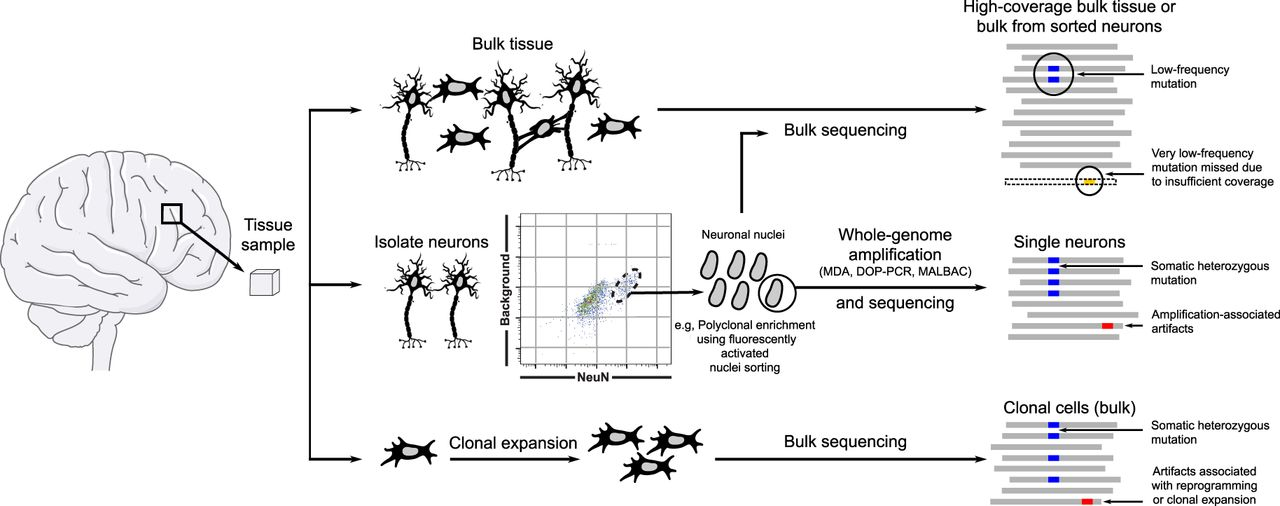
\includegraphics[width=0.9\textwidth]{figures/bsm-science-fig2.jpg}
\item<2->
\emph{case sample}\\
muscle cells \tikz[baseline=-0.5ex] \draw[->] (0,0) -- node[above] (A)
{pipeline} (1.5,0); \texttt{control.bam}
\end{enumerate}
\end{frame}

\begin{frame}{Hypothetical case}
\begin{columns}[t]
\begin{column}{0.5\textwidth}

TNseq.Mutect2
\begin{itemize}
\item TLOD---log odds for case sample
\item NLOD---log odds for control sample
\end{itemize}

\end{column}

\begin{column}{0.5\textwidth}

strelka2Somatic

\end{column}
\end{columns}
\end{frame}


\end{document}


\begin{columns}[t]
\begin{column}{0.5\textwidth}

\end{column}

\begin{column}{0.5\textwidth}

\end{column}
\end{columns}
